\documentclass[11pt,a4paper]{article}
\usepackage[T1]{fontenc}
\usepackage{lmodern}
\usepackage[margin=25mm]{geometry}
\usepackage{amsmath,amssymb}
\usepackage{graphicx}
\usepackage{booktabs}
\usepackage{siunitx}
\usepackage{caption}
\usepackage[hidelinks]{hyperref}
\usepackage{microtype}
\captionsetup{font=small,labelfont=bf}
\sisetup{detect-all}
\graphicspath{{figs/}}

\title{Downforce loss of a ground-effect wing in a wake is a dynamic-pressure effect:\\
validated 2D CFD and a comparison of surrogate models}
\author{Basil Mehmood\\[2pt]
\small Independent researcher, Pakistan\\
\small \href{mailto:basilmehmood117@gmail.com}{basilmehmood117@gmail.com}}
\date{Preprint, November 2026}

\begin{document}
\maketitle

\begin{abstract}
A ground-effect wing in a wake keeps its clean-air lift coefficient based on the dynamic pressure it actually meets: in our simulations the drop in that dynamic pressure explains a median 97\,\% of the downforce loss. We study the single-element wing of Zerihan and Zhang with two-dimensional steady RANS (OpenFOAM, $k$-$\omega$ SST), impose a parametric wake at the inlet, and measure the flow the wing meets with an empty-domain probe. The set-up is validated against Zerihan's wind-tunnel data and published CFD, with a discretisation uncertainty below 1\,\% (Grid Convergence Index). Across 56 cases, ride height ($h/c = 0.2$--$0.5$) and wake width change retention by less than 1\,\% once the dynamic pressure at the wing is known; wake turbulence partly offsets the loss, adding 4--9\,\% downforce at 5--8\,\% turbulence intensity at the wing at the cost of higher pressure drag. Of seven models compared by leave-one-out validation, a Gaussian-process surrogate predicts retention best (RMSE 0.007), ahead of a tuned neural network (0.012), a two-constant physics rule (0.014) and tree ensembles (0.03--0.04); the no-fit rule ``retention equals the dynamic-pressure ratio at the wing'' already reaches $R^2 = 0.985$. Sobol indices assign the variance to the wake deficit and its vertical offset, both acting through the dynamic pressure at the wing. The results reduce wake sensitivity to one measurable quantity and provide a cheap, validated surrogate for wake studies on modest hardware.
\end{abstract}

\noindent\textbf{Keywords:} ground effect; wing in a wake; motorsport aerodynamics; RANS; surrogate modelling; Gaussian process; sensitivity analysis

\section{Introduction}
A car following closely loses downforce in the wake of the car ahead, which is the main aerodynamic barrier to overtaking in Formula~1. The 2022 regulations were designed to reduce this loss: the pre-season projection was 4\,\% at 20\,m and 18\,\% at 10\,m for the 2022 car, against 35\,\% and 47\,\% for the 2021 car \cite{f1_2021}. Later FIA two-car CFD, reported by the press, puts the 2025 cars back at about 20\,\% at 20\,m and 35\,\% at 10\,m \cite{race_2025}.

Wind-tunnel and CFD studies show what a wing or car loses in an idealised wake \cite{newbon2017,soso2006,guerrero2020}, but each covers only a few wake settings because the simulations and tests are expensive. Three questions remain open: which features of the wake matter, whether ride height changes a wing's sensitivity to the wake, and how well cheap surrogate models can stand in for the CFD. This paper makes three contributions:
\begin{enumerate}
\item A validated, laptop-scale 2D CFD study of a ground-effect wing in a parametric wake that separates the wake's velocity deficit, turbulence, vertical position and width from the wing's ride height, using an empty-domain probe of the flow the wing actually meets.
\item A test of a simple law, that downforce retention equals the dynamic-pressure ratio at the wing, with the separate effects of turbulence, ride height and wake shape quantified against it.
\item A comparison of surrogate-model families (Gaussian process, neural network, tree ensembles, polynomial regression and physics-based rules) on the resulting data with leave-one-out validation, followed by a Sobol sensitivity analysis.
\end{enumerate}
All simulations ran on a four-core laptop; the code and results are released (see Data availability).

\section{Related work}
\textbf{Wings in ground effect.} Zerihan measured a Tyrrell-026-derived single-element wing and a two-element wing over a moving ground, reporting forces, surface pressures, wake surveys and 2D CFD \cite{zerihan2001,zerihan2000,zhang2003}. These data are the validation basis here.

\textbf{Wings and cars in wakes.} Newbon et al.\ \cite{newbon2017} found that the dynamic-pressure deficit accounts for as much as 90\,\% of the front-wing downforce loss on the centreline at one car length; upwash was a smaller effect, and downforce recovered with a lateral offset of about half a car width. Soso and Wilson \cite{soso2006} measured a wing in ground effect behind generic racing-car wakes, and Guerrero and Castilla \cite{guerrero2020} simulated a complete Formula~1 car in a wake, finding downforce losses of 23--62\,\%. The FIA's two-car straight-line CFD gives downforce retained at fixed gaps for successive rule sets \cite{f1_2021,race_2025}; these figures assume identical, aligned cars on a straight.

\textbf{Race data.} Joshi \cite{joshi2026} analysed 100{,}486 laps from 2021--2025 and found no statistically significant change in the lap-time penalty of following after the 2022 regulations. A wing-level law such as the one reported here offers one way to interpret why aerodynamic gains need not appear in lap time.

\textbf{Surrogates in motorsport aerodynamics.} Recent work uses a physics-informed neural network for front-wing coefficients \cite{shah2025} and a graph-based neural operator trained on RANS data of a parametric LMP2 car \cite{thumiger2026}. Direct comparisons of surrogate families on small CFD datasets with honest leave-one-out validation are rare.

\section{Method}
\subsection{Geometry, domain and boundary conditions}
The profile is Zerihan's single-element wing at its reference incidence of $1^\circ$ (Table~2 of \cite{zerihan2001}; chord $c = 223.4$\,mm, blunt trailing edge). The two-dimensional domain extends $5c$ upstream, $12c$ downstream and $5c$ above the ground (Fig.~\ref{fig:setup}a) and is one cell thick. Ride height $h$ is measured from the ground to the lowest point of the wing. The ground moves at $U_\infty = 30$\,m/s; the wing is a no-slip wall; the top is a slip wall and the outlet is at fixed pressure. The chord Reynolds number is $4.5\times10^5$.

\begin{figure}[t]
\centering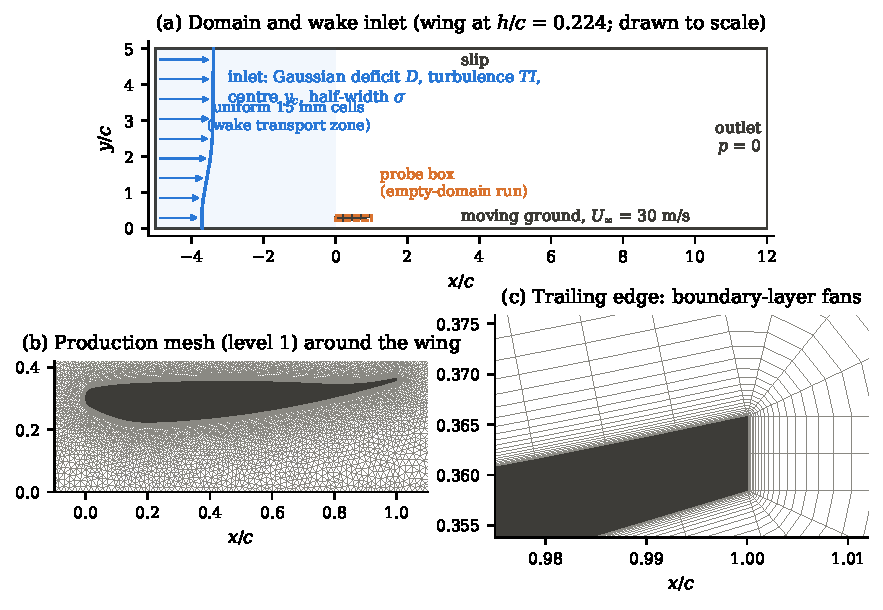
\includegraphics[width=\textwidth]{fig1_setup}
\caption{(a) Domain, wake inlet and probe box, to scale. (b) Production (level-1) mesh around the wing at $h/c = 0.224$. (c) Boundary-layer fans at the blunt trailing edge.}
\label{fig:setup}
\end{figure}

\subsection{Mesh}
Hybrid meshes were generated with gmsh: a structured boundary layer on the wing (first cell \SI{15}{\micro\metre}, $y^+\approx1$, growth ratio 1.2, fans at both trailing-edge corners; Fig.~\ref{fig:setup}c) and triangles elsewhere, refined towards the wing, its wake and the ground. Three levels differ by a factor of 1.5 in surface and wake spacing. Level~1 (41--45k cells) is the production mesh; for wake cases, a zone of uniform 15\,mm cells between the inlet and the wing (52k cells in total) carries the imposed profile to the wing without numerical smearing.

\subsection{Solver and convergence}
The steady incompressible RANS equations are solved with simpleFoam (OpenFOAM v2512) and the $k$-$\omega$ SST model, using linearUpwind convection for velocity and limitedLinear for $k$ and $\omega$, with under-relaxation factors of 0.7 (velocity), 0.6 (turbulence) and 0.5 (pressure). Each case runs for 2000 iterations; a case is accepted when $C_L$ changes by less than 0.5\,\% over the last 500. Forces are integrated from the wall pressure, so $C_D$ denotes pressure drag $C_{D,p}$. Downforce is reported as a positive $C_L$.

\subsection{Wake inlet and empty-domain probe}
The leading car's wake is imposed as a Gaussian deficit in streamwise velocity with a turbulence intensity that peaks at the wake centre:
\begin{equation}
U(y) = U_\infty\left[1 - D\,e^{-(y-y_c)^2/2\sigma^2}\right],\qquad
Tu(y) = 0.005 + (TI - 0.005)\,e^{-(y-y_c)^2/2(1.5\sigma)^2},
\end{equation}
with $k = 1.5\,(U\,Tu)^2$ and $\omega = \sqrt{k}/(C_\mu^{1/4}\ell)$, $\ell = 0.05$\,m, imposed through \texttt{timeVaryingMappedFixedValue}. The wake centre sits $dy$ above the wing's mid-height, $y_c = h + 0.071c + dy$.

Because the imposed profile evolves on its way to the wing, every wake is also run through the same domain without the wing. The flow is averaged over the box the wing would occupy ($0 \le x \le c$, $h \le y \le h + 0.142c$) to give the dynamic-pressure ratio $q_{wing}/q_\infty = \overline{|U|^2}/U_\infty^2$, the mean flow angle, the turbulence intensity reaching the wing and the shear across the wing. Results are expressed in terms of what the wing actually meets.

\textbf{Upwash.} An imposed inlet upwash of $3^\circ$ arrived at the wing as $0.07^\circ$: in 2D above a ground plane, continuity ($\partial V/\partial y = -\partial U/\partial x$) does not allow a vertical velocity to persist, and with an open top boundary the flow escaping upwards deepened the deficit at the wing from 20 to 28\,\%. Upwash at a following car's wing comes from the leading car's trailing vortices, a 3D effect, so it is excluded.

\subsection{Retention and campaign design}
Retention is $R = C_L / C_{L0}(h)$, where $C_{L0}(h)$ is a quadratic fit to four clean-air runs at $h/c = 0.2$, 0.3, 0.4 and 0.5 on the same mesh. The campaign comprises those 4 clean runs; 12 one-factor-at-a-time runs around $h/c = 0.224$ with a wake centred on the wing (deficit $D = 0.1$, 0.2, 0.3; $TI = 3$, 6, 10\,\%; offset $dy/c = 0.5$, 1, 2 and $h/c = 0.3$, 0.4, 0.5 at $D = 0.2$); and a 40-point Latin hypercube over $D \in [0.05, 0.30]$, $TI \in [0.5, 10]\,\%$, $h/c \in [0.2, 0.5]$ and $dy/c \in [0, 2]$, with $\sigma = c$. Additional runs checked the wake width ($\sigma/c = 0.5$, 2) and the inlet length scale ($\ell = 0.01$, 0.10\,m).

\subsection{Surrogate models and sensitivity}
Seven models of $R$ were compared, each scored by leave-one-out cross-validation over the 56 cases. Data-driven models use the four design inputs $(D, TI, h/c, dy/c)$: a Gaussian process (GP) with an anisotropic Mat\'ern-5/2 kernel and a white-noise term; a multilayer perceptron whose size and weight decay are chosen by an inner five-fold search inside each fold; quadratic ridge regression; a random forest; and gradient boosting. Two physics rules use the probe instead: $R = q_{wing}/q_\infty$ with no fitted constant, and $R = a\,q + b\,q\,(TI_{wing} - 0.005)$. First-order and total Sobol indices of $R$ were computed on the GP with Saltelli sampling ($2048 \times 6$ evaluations) over the campaign ranges.

\section{Verification and validation}
Table~\ref{tab:gci} summarises the mesh study. Each finer mesh was started from the coarser solution and run for 3000 iterations; every run settled. At $h/c = 0.448$ convergence is monotonic with observed order $p = 2.41$ and $\mathrm{GCI_{fine}} = 0.19\,\%$ \cite{celik2008}; level~1 lies 0.7\,\% above the extrapolated value. At $h/c = 0.224$ convergence is oscillatory and, following \cite{celik2008}, we report the spread (0.6\,\%) as the uncertainty. The production mesh therefore adds less than 1\,\% numerical uncertainty.

\begin{table}[t]
\centering\small
\caption{Mesh independence (single-element wing). Cells and $C_L$ on levels 1/2/3.}
\label{tab:gci}
\begin{tabular}{lccl}
\toprule
$h/c$ & Cells (k) & $C_L$ & Result \\
\midrule
0.448 & 44.6 / 79.8 / 154.3 & 1.1384 / 1.1345 / 1.1324 & $p = 2.41$, $C_{L,ext} = 1.1307$, GCI$_{fine}$ = 0.19\,\% \\
0.224 & 40.8 / 72.6 / 137.6 & 1.4134 / 1.4181 / 1.4097 & oscillatory, spread 0.6\,\% \\
\bottomrule
\end{tabular}
\end{table}

Figure~\ref{fig:val} compares clean-air $C_L$ with Zerihan's measurements and 2D CFD. The present results lie between Zerihan's $k$-$\omega$ and Spalart--Allmaras solutions at every height and within 5\,\% of both for $h/c \ge 0.18$ (Table~\ref{tab:val}). Against the wing-centre pressures, the difference moves from $-4\,\%$ at $h/c = 0.18$ to $+11\,\%$ at 0.45; a likely reason is that finite-span downwash, absent in 2D, weakens close to the ground. The ground-effect gain $C_L(0.224)/C_L(0.448)$ is 1.24, against 1.19 and 1.26 for Zerihan's two RANS models and 1.28--1.37 in the experiments. Below $h/c \approx 0.11$ the solution shows signs of trailing-edge separation and the case at $h/c = 0.067$ did not converge; the validated range is $h/c \ge 0.2$. Because retention is a ratio at fixed height, a constant 2D offset largely cancels in the quantities studied below.

\begin{figure}[t]
\centering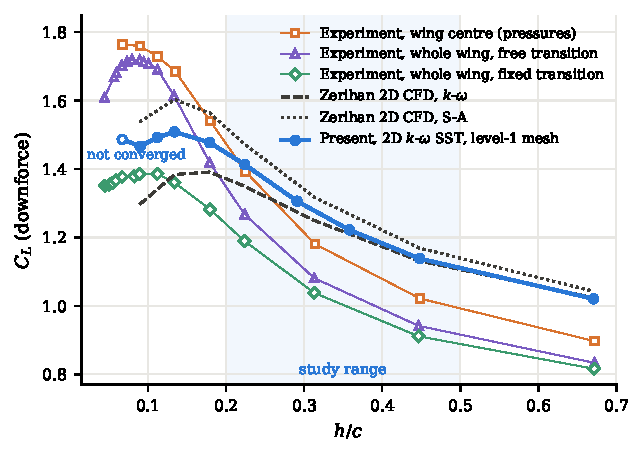
\includegraphics[width=0.72\textwidth]{fig2_validation}
\caption{Clean-air downforce against ride height: present 2D RANS (level-1 mesh), Zerihan's measurements \cite{zerihan2001} and his 2D CFD. Experimental and reference values were digitised from the 300\,dpi thesis scan (uncertainty about $\pm0.003$ in $C_L$).}
\label{fig:val}
\end{figure}

\begin{table}[t]
\centering\small
\caption{Clean-air validation: present $C_L$ and its difference from Zerihan's 2D CFD and wing-centre experiment.}
\label{tab:val}
\begin{tabular}{ccccc}
\toprule
$h/c$ & $C_L$ & vs $k$-$\omega$ CFD & vs S--A CFD & vs experiment (centre) \\
\midrule
0.134 & 1.509 & +9.0\,\% & $-5.9$\,\% & $-10.6$\,\% \\
0.179 & 1.477 & +6.2\,\% & $-5.5$\,\% & $-4.2$\,\% \\
0.224 & 1.413 & +4.7\,\% & $-4.0$\,\% & +1.2\,\% \\
0.291 & 1.306 & +2.5\,\% & $-3.7$\,\% & +5.7\,\% \\
0.358 & 1.222 & +1.0\,\% & $-3.6$\,\% & +8.3\,\% \\
0.448 & 1.138 & +0.6\,\% & $-2.6$\,\% & +11.4\,\% \\
0.671 & 1.021 & $-0.3$\,\% & -- & +13.7\,\% \\
\bottomrule
\end{tabular}
\end{table}

\section{Results}
\subsection{Retention follows the dynamic pressure at the wing}
All 56 cases converged. The clean runs on the wake-transport mesh agree with the validation sweep to within 1\,\%. Figure~\ref{fig:flow} shows the velocity field for clean air, a 20\,\% deficit centred on the wing, and 10\,\% inlet turbulence. In the wake case, the flow pattern is that of clean air scaled down: the acceleration under the wing and the near wake keep their shape while the velocities fall.

\begin{figure}[t]
\centering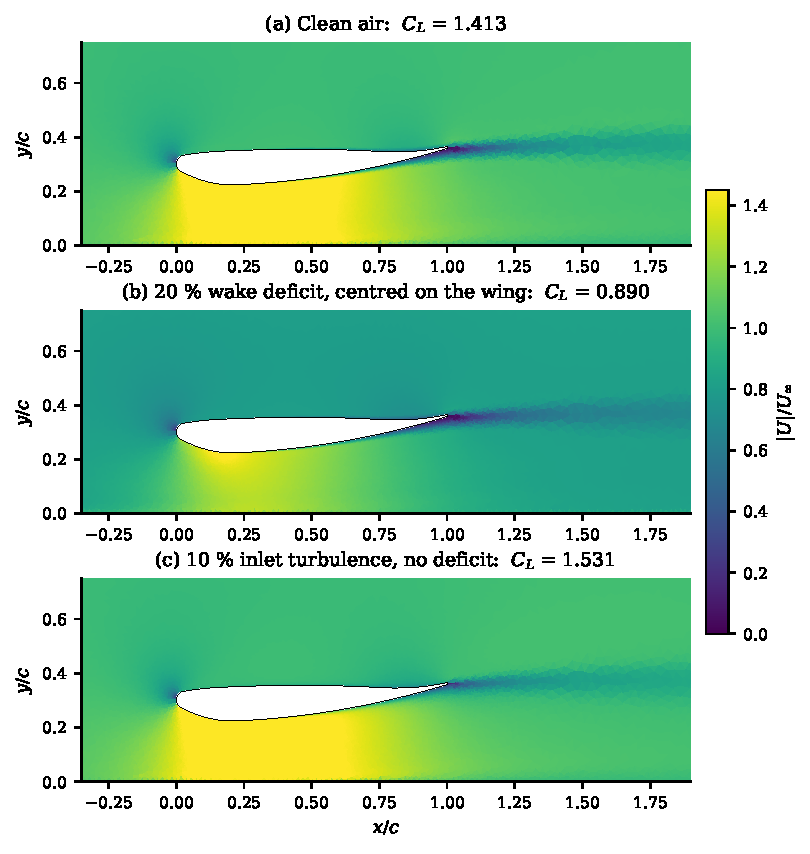
\includegraphics[width=0.88\textwidth]{fig3_flow}
\caption{Velocity magnitude around the wing at $h/c = 0.224$: (a) clean air, (b) 20\,\% deficit centred on the wing, (c) 10\,\% inlet turbulence ($\ell = 0.05$\,m) without deficit.}
\label{fig:flow}
\end{figure}

Retention follows the dynamic-pressure ratio measured by the probe (Fig.~\ref{fig:ret}a): over all 52 wake cases the median of $R/(q_{wing}/q_\infty)$ is 0.995, and in cases losing more than 2\,\% the dynamic-pressure drop explains a median 97\,\% of the loss (inter-quartile range 95--103\,\%). Pressure drag follows the same law: $C_{D,p}/(q_{wing}/q_\infty) = 0.0191$, 0.0195 and 0.0199 at $D = 0.1$, 0.2 and 0.3, against 0.019--0.020 in clean air.

\begin{figure}[t]
\centering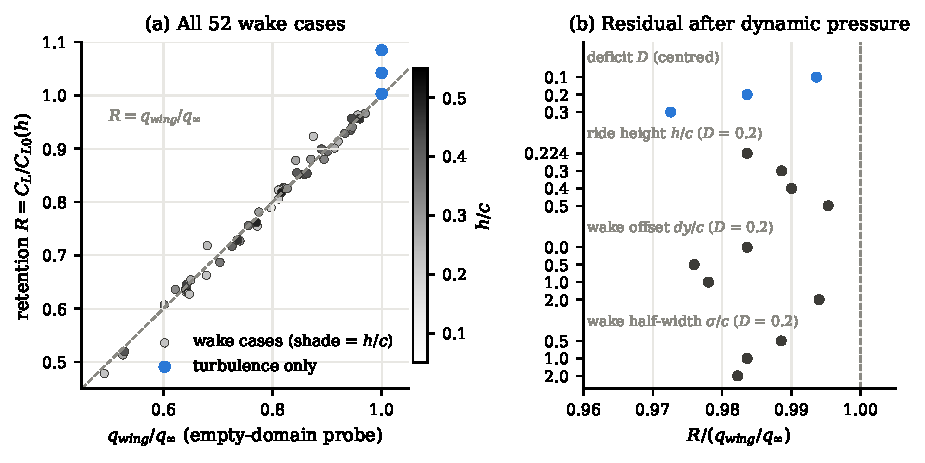
\includegraphics[width=\textwidth]{fig4_retention}
\caption{(a) Retention against the dynamic-pressure ratio at the wing for all wake cases; dashed line $R = q_{wing}/q_\infty$. (b) Remaining ratio $R/(q_{wing}/q_\infty)$ in the one-factor-at-a-time runs.}
\label{fig:ret}
\end{figure}

What is left after dynamic pressure is small (Fig.~\ref{fig:ret}b). Retention falls slightly below the dynamic-pressure ratio as the deficit grows ($R/q = 0.994$, 0.984 and 0.973 at $D = 0.1$, 0.2, 0.3). In the same 20\,\% wake, retention is 0.631, 0.634, 0.635 and 0.638 at $h/c = 0.224$, 0.3, 0.4 and 0.5 against a dynamic-pressure ratio of 0.642: a wing running lower does not lose a larger fraction. Changing the wake half-width from $0.5c$ to $2c$ moves $R$ from 0.638 to 0.629, and moving the wake centre above the wing matters only through the deficit that reaches it. A regression of $R/q - 1$ on the probed quantities finds a significant effect of turbulence at the wing (coefficient 0.76, $p < 10^{-8}$) and a weak effect of shear (0.11, $p = 0.02$), and none of ride height ($p = 0.07$).

\subsection{Turbulence raises downforce}
Without a velocity deficit, downforce rises with the turbulence that reaches the wing (Fig.~\ref{fig:turb}): $+0.3\,\%$ at 2.7\,\% turbulence intensity at the wing, $+4.2\,\%$ at 4.9\,\% and $+8.6\,\%$ at 7.2\,\%. The inlet length scale controls how much turbulence survives to the wing; at 10\,\% inlet intensity the gain is $+5.6$, $+8.6$ and $+8.3\,\%$ for $\ell = 0.01$, 0.05 and 0.10\,m. The two highest-turbulence cases were rerun for 4000 iterations to confirm convergence. Pressure drag rises with turbulence ($C_{D,p}$ from 0.019 to 0.025), so the gain is not a suppression of separation; Fig.~\ref{fig:flow}c shows a shallower near wake behind the trailing edge. We report the effect as a model result, $+4$ to $+9\,\%$ at 5--8\,\% turbulence at the wing, that requires experimental confirmation.

\begin{figure}[t]
\centering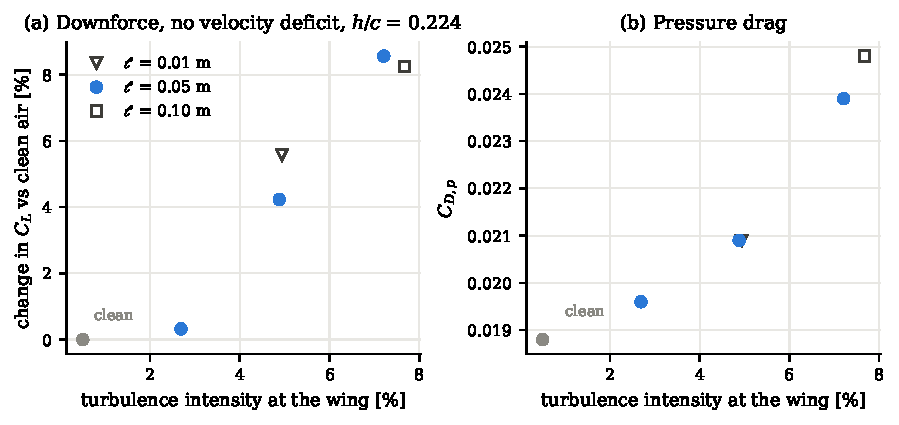
\includegraphics[width=\textwidth]{fig5_turbulence}
\caption{Effect of wake turbulence without velocity deficit at $h/c = 0.224$: (a) change in $C_L$ and (b) pressure drag against the turbulence intensity reaching the wing, for three inlet length scales.}
\label{fig:turb}
\end{figure}

\subsection{Surrogate models and sensitivity}
Table~\ref{tab:models} and Fig.~\ref{fig:models}a compare the models. The Gaussian process is the most accurate (LOO RMSE 0.0073, $R^2 = 0.9975$), followed by the tuned neural network (0.0116). The two-constant physics rule (0.0139) is close to the black-box models, and even the no-fit rule $R = q_{wing}/q_\infty$ reaches $R^2 = 0.985$; its largest errors are the turbulence-only cases. Tree ensembles, which build piecewise-constant fits, perform worst on these 56 smooth samples.

\begin{table}[t]
\centering\small
\caption{Leave-one-out accuracy of retention models (56 cases).}
\label{tab:models}
\begin{tabular}{llccc}
\toprule
Model & Inputs & RMSE & Max.\ error & $R^2$ \\
\midrule
Gaussian process (Mat\'ern 5/2, ARD) & $D, TI, h/c, dy/c$ & 0.0073 & 0.027 & 0.9975 \\
Neural network (nested tuning) & $D, TI, h/c, dy/c$ & 0.0116 & 0.039 & 0.9936 \\
Physics: $R = a q + b q (TI_{wing} - 0.005)$ & probe & 0.0139 & 0.060 & 0.9908 \\
Quadratic ridge regression & $D, TI, h/c, dy/c$ & 0.0155 & 0.043 & 0.9886 \\
Physics: $R = q_{wing}/q_\infty$ (no fit) & probe & 0.0180 & 0.085 & 0.9845 \\
Gradient boosting & $D, TI, h/c, dy/c$ & 0.0326 & 0.099 & 0.9495 \\
Random forest & $D, TI, h/c, dy/c$ & 0.0391 & 0.095 & 0.9274 \\
\bottomrule
\end{tabular}
\end{table}

\begin{figure}[t]
\centering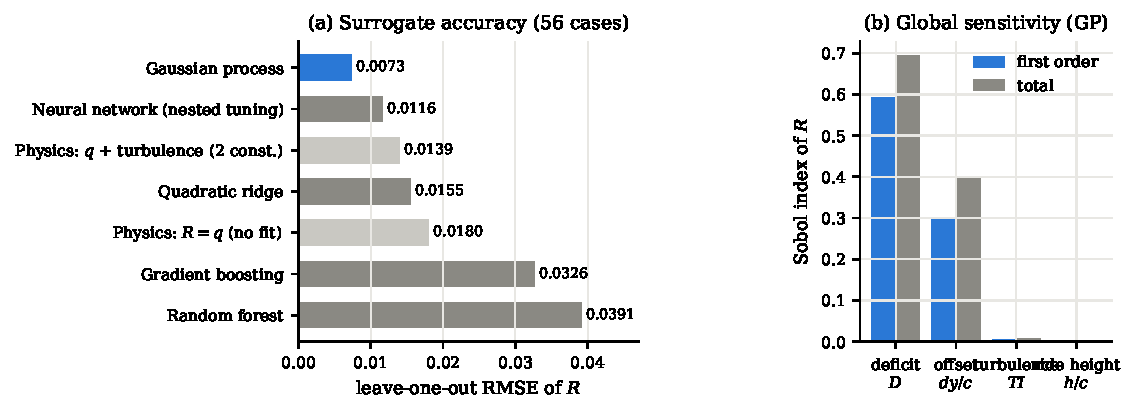
\includegraphics[width=\textwidth]{fig6_models}
\caption{(a) Leave-one-out RMSE of retention by model. (b) First-order and total Sobol indices of retention from the Gaussian process.}
\label{fig:models}
\end{figure}

The Sobol indices (Fig.~\ref{fig:models}b) attribute the variance of $R$ to the deficit (first-order 0.59, total 0.69) and the wake offset (0.30, 0.40); turbulence (0.005, 0.008) and ride height (0.000, 0.002) are negligible over these ranges. Deficit and offset matter because together they set the dynamic pressure at the wing; turbulence's index is small because its effect, though up to 9\,\%, is small next to deficits of up to 30\,\%.

\section{Discussion}
To first order, downforce loss in a wake is a dynamic-pressure effect. The wing keeps its clean-air coefficient based on the local dynamic pressure to within 1--3\,\%; its ride height does not change the fractional loss; and the wake's shape and position matter only through the deficit that reaches the wing. For a following car, the quantity to predict is therefore the dynamic pressure at the front wing rather than the gap or the wake's own parameters. If a whole car behaved like this wing, fixed-gap figures such as 15\,\% loss at 10\,m for the 2022 baseline car \cite{race_2025} would translate directly into an effective dynamic-pressure ratio, and anything that moves a car out of the wake core, such as a lateral offset \cite{newbon2017}, would reduce the loss in proportion to the dynamic pressure it recovers.

Practical implications follow. Wake-sensitivity studies should report the dynamic pressure at the wing from an empty-domain probe, since a no-fit rule based on it explains 98.5\,\% of the variance. Clean-air ride-height data can be reused for dirty air by scaling with that dynamic pressure, to within about 1\,\% over $h/c = 0.2$--0.5. For small, smooth CFD datasets, Gaussian processes should be preferred to tree ensembles; tuned neural networks are competitive but less accurate.

\textbf{Limitations.} The study uses 2D steady RANS with a fully turbulent $k$-$\omega$ SST model, so tip vortices, upwash and transition are absent, and only one incidence is studied; the turbulence gain is a model result that depends on the assumed length scale. Only the single-element wing is used: a two-element wing in 2D was 25--45\,\% above the experiment, consistent with its low aspect ratio. The wake is an idealised Gaussian deficit centred at or above the wing, whereas real wakes also carry vortices and lateral structure. Experimental and reference data were digitised from the thesis figures ($\pm0.003$ in $C_L$; digitised values are released with the code).

\textbf{Future work.} Three-dimensional simulation of a front wing with lateral wake offset and trailing vortices; wind-tunnel tests of the turbulence effect; and comparison with real following behaviour from race data, subject to data permissions.

\section{Conclusions}
Downforce loss of a ground-effect wing in a wake is set by the dynamic pressure the wing meets: ride height and wake shape matter little, turbulence partly offsets the loss, and a Gaussian-process surrogate trained on 56 laptop-scale simulations reproduces the CFD to 0.007 in retention.

\section*{Data and code availability}
All scripts (meshing, case set-up, probe, analysis, surrogates) and the CFD results tables are available at \url{https://github.com/Basil-117/ground-effect-F1wing-wake}. The simulations use OpenFOAM v2512, gmsh, scikit-learn, SALib and statsmodels.

\section*{Declarations}
\textbf{Funding:} This research received no external funding. \textbf{Competing interests:} The author declares no competing interests.

\begin{thebibliography}{99}\small
\bibitem{celik2008} I.~B. Celik, U.~Ghia, P.~J. Roache, C.~J. Freitas, Procedure for estimation and reporting of uncertainty due to discretization in CFD applications, \emph{Journal of Fluids Engineering} 130(7) (2008) 078001. doi:10.1115/1.2960953.
\bibitem{f1_2021} Formula~1, 10 things you need to know about the all-new 2022 F1 car, formula1.com, 15 July 2021.
\bibitem{guerrero2020} A.~Guerrero, R.~Castilla, Aerodynamic study of the wake effects on a Formula~1 car, \emph{Energies} 13(19) (2020) 5183.
\bibitem{joshi2026} B.~Joshi, The persistence of the dirty air penalty: a causal analysis of Formula~1's 2022 ground effect regulations, arXiv:2608.03192 (2026).
\bibitem{newbon2017} J.~Newbon, D.~Sims-Williams, R.~Dominy, Aerodynamic analysis of Grand Prix cars operating in wake flows, \emph{SAE International Journal of Passenger Cars -- Mechanical Systems} 10(1) (2017) 318--329. doi:10.4271/2017-01-1546.
\bibitem{race_2025} J.~Noble, Exclusive: new data on F1 aero losses ruining close racing, \emph{The Race}, 26 November 2025.
\bibitem{shah2025} N.~Shah, Computational fluid dynamics optimization of F1 front wing using physics informed neural networks, arXiv:2509.01963 (2025).
\bibitem{soso2006} M.~D. Soso, P.~A. Wilson, Aerodynamics of a wing in ground effect in generic racing car wake flows, \emph{Proc.\ IMechE Part D: Journal of Automobile Engineering} 220(1) (2006) 1--13. doi:10.1243/095440705X69632.
\bibitem{thumiger2026} N.~Thumiger, A.~Bartezzaghi, M.~Rigotti, C.~Skura, T.~Frick, E.~Serioli, F.~Arbucci, A.~C.~I. Malossi, Faster by design: interactive aerodynamics via neural surrogates trained on expert-validated CFD, arXiv:2604.18491 (2026).
\bibitem{zerihan2001} J.~Zerihan, An investigation into the aerodynamics of wings in ground effect, PhD thesis, University of Southampton (2001).
\bibitem{zerihan2000} J.~Zerihan, X.~Zhang, Aerodynamics of a single element wing in ground effect, \emph{Journal of Aircraft} 37(6) (2000) 1058--1064.
\bibitem{zhang2003} X.~Zhang, J.~Zerihan, Aerodynamics of a double-element wing in ground effect, \emph{AIAA Journal} 41(6) (2003) 1007--1016.
\end{thebibliography}
\end{document}
